\documentclass[tikz]{standalone}
\usepackage{amsmath,amssymb}
\newcommand{\la}[1]{\boldsymbol{#1}}
\usepackage{pgf}
\usepackage{tikz}
\usetikzlibrary{arrows,automata,positioning}
\tikzset{
    state/.style={
           rectangle,
           rounded corners,
           draw=black, semithick,
           minimum height=2em,
           minimum width=5em,
           inner sep=2pt,
           text centered,
           },
}



\usepackage[latin1]{inputenc}
\begin{document}
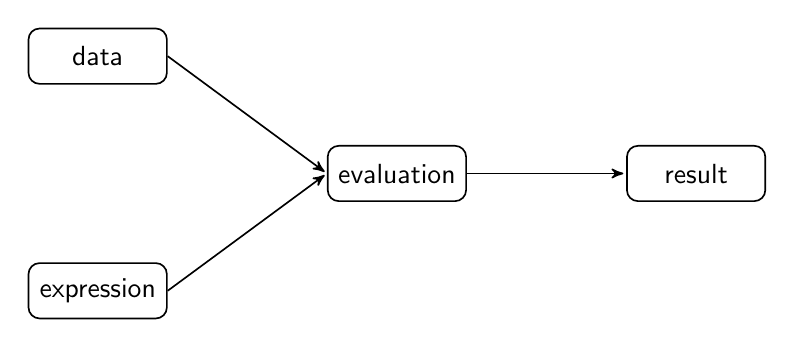
\begin{tikzpicture}[->,>=stealth',shorten >=1pt,auto,
                    node distance=3.8cm,
                    semithick]

  \node[state]     (A)              {\textsf{data}};
  \node[draw=none] (B) [below = 1cm of A] {};
  \node[state]     (C) [below = 1cm of B] {\textsf{expression}};
  \node[state]     (D) [right of=B] {\textsf{evaluation}};
  \node[state]     (E) [right of=D] {\textsf{result}};
 
  \path (A.east) edge (D.west); 
  \path (C.east) edge (D.west);
  \path (D) edge (E);

\end{tikzpicture}

\end{document}
